%****************************************************************************%
%* DIET User's Manual Multi-MA chapter file                                 *%
%*                                                                          *%
%*  Author(s):                                                              *%
%*    - Sylvain DAHAN (dahan@lifc.univ-fcomte.fr)                           *%
%*                                                                          *%
%* $LICENSE$                                                                *%
%****************************************************************************%
%* $Id$
%* $Log$
%* Revision 1.4  2006/12/19 08:31:21  ycaniou
%* Corrections
%*
%* Revision 1.3  2006/12/19 00:06:41  ecaron
%* Take into account multima.fig
%*
%****************************************************************************%
\chapter{Multi-MA extension}
\label{ch:multiMAextension}

The hierarchical organization of \diet is efficient when the set of
resources is shared by few individuals. However, the aim of grid
computing is to share resources between several individuals. In that
case, the \diet hierarchy become inefficient. The Multi-MA extension
has been implemented to resolve this issue. This chapter explains the
different scalability issues of grid computing and how to use the
multi-MA extension to deal with them.

\section{Function of the Multi-MA extension}

The use of a monolithic architecture become more and more difficult
when the number of users and the number of resources grow
simultaneously. When a user tries to resolve a problem, without the
multi-MA extension, \diet looks for the better \sed that can solve
it. This search involves the fact that each \sed has to be queried to
run a performance prediction as described in section~\ref{sec:solvepb}.

The need to query every \sed that can resolve a problem is a serious
scalability issue. To avoid it, the multi-MA extension proposes to
interconnect several MA together. So, instead of having the whole set
of \sed available under a hierarchy of a unique MA, there are several
MA and each MA manages a subset of {\sed}s. Those MA are
interconnected in a way that they can share the access to their
{\sed}s.

Each MA works like the usual: when they received a query from a user,
they looks for the best \sed which can resolve their problem inside
their hierarchy. If there is no \sed available in its hierarchy, the
queried MA forwards the query to another MA to find a \sed that can be
used by its client. This way, \diet is able to support more clients
and more servers because each client request is forwarded to a number
of {\sed}s that is independent of the total number of available
{\sed}s.

\section{Deployment example}

The instructions about how to compile \diet with the multi-MA
extension are available in section~\ref{sec:multimainstall} and the
configuration instructions are available in
section~\ref{sec:multimaconfig}.

The example described here is about four organizations which want to
share there resources. The first organization, named alpha, have ten
{\sed}s which give access to the service \textbf{a}. The second
organization, named beta, have eight {\sed}s with the service
\textbf{a} and three with the service \textbf{b}. The third one, named
gamma, have two {\sed}s with the service \textbf{c}.  The last one,
named delta, have one \sed with the service \textbf{a}, but the server
crash and the \sed is unavailable.

Each organization has it's own \diet hierarchy. All MAs (one for each
organization) are connected with the multi-MA extension as shown in
Figure~\ref{fig:multima}


\begin{figure}[h]
 \begin{center}
   \resizebox{.7\linewidth}{!}{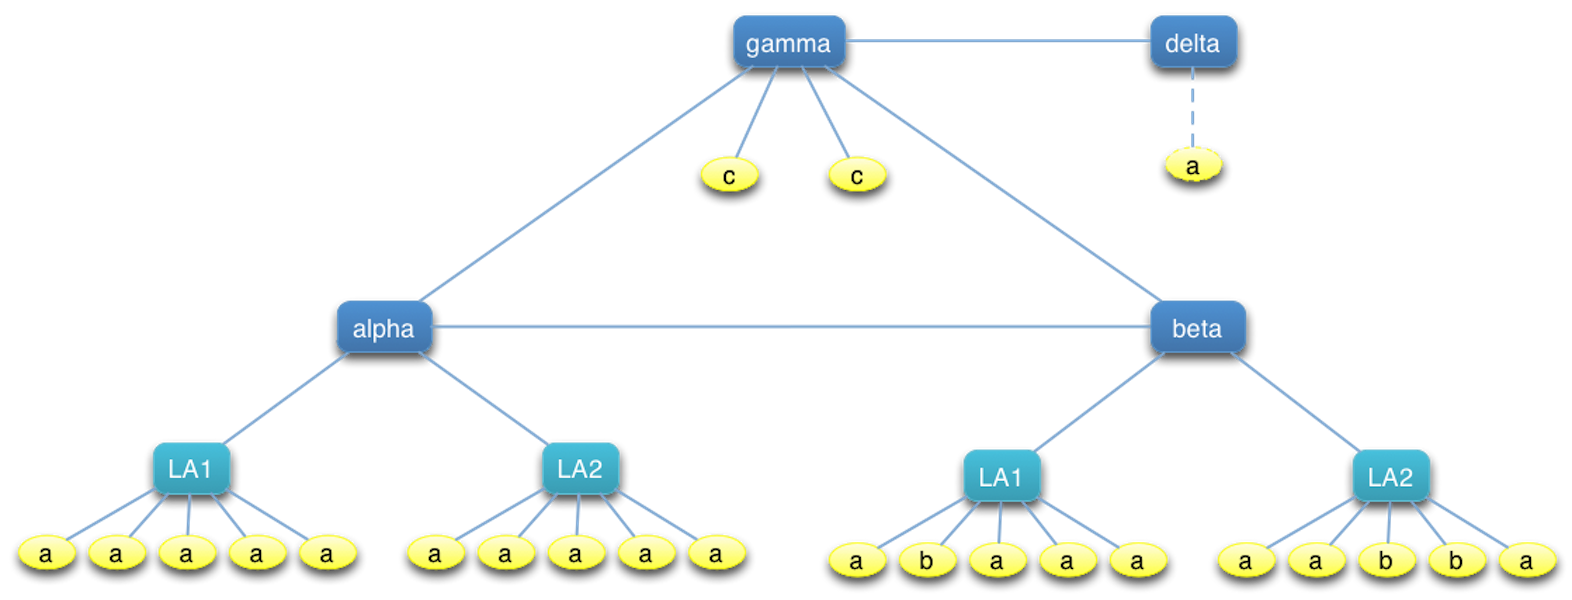
\includegraphics{fig/multima.eps}}
   \label{fig:multima}
  \caption{Example of a multi-MA deployment}
 \end{center}
\end{figure}

The following lines appear in the MA configuration file of alpha. They
tell that the multi-MA extension should listen for incoming connection
at port 2001. They also tell that the MA should create a link toward
the MA of the organization gamma and toward the MA of the organization
beta. (The description of each configuration parameter are available
in section~\ref{sec:multimaconfig}.)

\begin{verbatim}
agentType = DIET_MASTER_AGENT
dietHostname = diet.alpha.com
bindServicePort = 2001
neighbours = diet.beta.com:2001,ma.gamma.com:6000
\end{verbatim}

The following lines appear in the MA configuration file of beta:

\begin{verbatim}
agentType = DIET_MASTER_AGENT
dietHostname = diet.beta.com
bindServicePort = 2001
neighbours = diet.alpha.com:2001,ma.gamma.com:6000
\end{verbatim}

The following lines appear in the MA configuration file of gamma. The
\texttt{neighbours} value is empty. This means that the gamma's MA
will not try to connect itself to other MA. However, the three others
are configured to be connected to gamma. So, after all, the gamma MA
is connected to the other three.

\begin{verbatim}
agentType = DIET_MASTER_AGENT
dietHostname = ma.gamma.com
bindServicePort = 6000
neighbours = 
\end{verbatim}

Finally the following lines appear in the MA configuration file of delta:

\begin{verbatim}
agentType = DIET_MASTER_AGENT
dietHostname = ma.delta.com
bindServicePort = 2001
neighbours = ma.gamma.com:6000
\end{verbatim}

\section{Search examples}

The following section explains how a \texttt{diet\_call} is managed
when used on the previous architecture.

If a client sends a \texttt{diet\_call} for the problem \textbf{a} to
the alpha's MA, the alpha's MA will return a reference of one of it's
\sed. However, if its scheduler (see section~\ref{ch:plugin}) says
that no \sed is available, it will forward the request to beta and
gamma. If beta has an available \sed, it will be used to resolve the
problem. If not, the request is forwarded to delta.

Now, if a client performs a \texttt{diet\_call} for the problem
\textbf{c} to the delta's MA, the delta MA does not have a \sed that
can resolve this problem. So, it forwards the request to gamma. If
gamma has no available \sed, the request is forwarded to alpha and
beta.
